\section{Пример отказа бутстрепа}

Предположим, что у нас имеются данные $X_1, X_2,\ldots, X_n$ из равномерного распределения на $(0, \theta)$. Оценка $\thetahat$ по методу максимума правдоподобия есть наибольшее значение выборки $X_{(n)}.$ Мы сгенерировали выборку из 50 равномерно распределённых чисел на $(0,1)$ и получили $\thetahat = 0.988.$ На левой части рисунка 7.11 показана гистограмма 2000 бутстреп репликаций оценки $\thetahat^*$, полученных с помощью выборок из данных с возвращением. На правой части наблюдаем 2000 репликаций параметрического бутстрепа, полученных при взятии выборок из равномерного распределения на $(0, \thetahat).$\footnote{подписи parametric и nonparametric на рисунке следует поменять местами --- прим.ред.} Ясно, что гистограмма слева есть плохая аппроксимация того, что мы видим на правой. Так, в случае левой гистограммы оказывается, что в $62\%$ репликаций $\thetahat^* = \thetahat$. Вообще говоря, легко показать, что $\text{Prob}(\thetahat^* = \thetahat) = 1 - (1 - 1/n)^n \rightarrow 1 - e^{-1} \approx .632$ когда $n \rightarrow \infty.$ Однако, в параметрическом случае правой гистограммы $\text{Prob}(\thetahat^* = \thetahat) = 0$.
\\~\\
\noindent
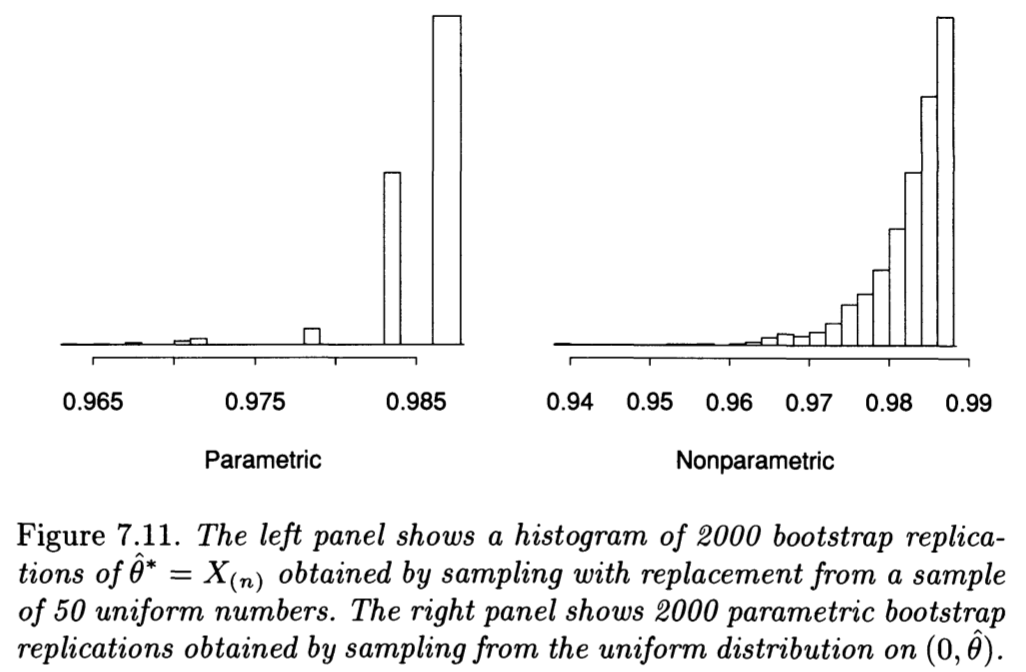
\includegraphics[width=0.9\linewidth]{6/f711.png}
\newline
\setcounter{table}{5} 
Что не так с непарамерическим бутстрепом? Сложность возникает потому, что эмпирическая функция распределения $\hat F$ не является хорошей оценкой настоящего распределения на его краях. Либо параметрические данные о $F$, либо некоторое сглаживание $\hat F$ необходимо для того, чтобы разрешить эту проблему. Детали и ссылки об этой проблеме можно найти в Beran и Ducharme (1991, с.23). Непараметрический бутстреп может отказать и в других примерах, где $\theta$ зависит от гладкости $F.$ К примеру, если $\theta$ есть число атомов у $F$, то $\thetahat = n$ будет плохой оценкой $\thetahat.$ 